\section{Анализ литературно патентных исследований}

% В данном разделе будет приведена информация про то что именно из
% себя представляет разрабатываемое устройство, а именно то,
% что оно является полётным контроллером.

% Также пять патентов схожих по параметрам
% устройств, выполняющих функции полётных контроллеров.

\subsection{Обзор методов 
  и средств управления  двигателями 
  мультироторных беспилотных летательных аппаратов}

В типичной системе контроля полета
мультироторного летательного аппарата
пять параметров подлежат отслеживанию: длина четырех управляющих
сервоприводами импульсов, которые контролируют тягу, крен, тангаж и
рысканье, и напряжение питания.

Управление скоростью вращения винтов квадрокоптера осуществляется
изменением уровня управляющих напряжений (или скважностью, если
управляющий сигнал широтно-импульсный). Как правило, двигатели
квадрокоптера — это двигатели постоянного тока, обладающие своей
динамикой ~\cite{liisuho}.
% % Лысухо Г.В., Масленников А.Л. Квадрокоптер: динамика и
% управление. Политехнический молодежный журнал, 2020, №
% 05(46). http://dx.doi.org/10.18698/2541-8009-2020-5-604


Наиболее часто в квадрокоптерах применяют бесколлекторные двигатели,
якорь которых представляет собой набор неодимовых магнитов, а статор
состоит из обмотки возбуждения, на который подается управляющее
напряжение. В отличие от коллекторных двигателей, где якорь вращается
внутри статора, у бесколлекторных якорь вращается постоянного тока
вокруг статора, который находится внутри~\cite{Solodovnikov1976}.
% Солодовников В.В., ред. Устройства и элементы систем автоматического
% регулирования. Техническая кибернетика. Кн. 3. Исполнительные
% устройства и сервомеха- низмы. М., Машиностроение, 1976.

Малогабаритные быстродействующие сервоприводы применяются в
современных высокоточных системах управления подвижными объектами:
рулевыми системами летательных аппаратов, автоматическими
манипуляторами, роботами с подвижными элементами конструкции и
др~\cite{dyakovSUBSTANTIATIONRELIABILITYSERVOMOTORS2023}.

Под сервоприводом в данной работе подразумевается вращающийся привод,
управляющий широтно-импульсной модуляцией, который за счёт обратной
связи позволяет точно контролировать вал сервопривода, поворачивая его
на заданный угол или поддерживая определенную скорость или ускорение.

Говоря кратко, разрабатываемое изделие, можно назвать одним
общепринятым словом — полётный контроллер.

Полётный контроллер выполнен в виде платы, на которую, с помощью
монтажа в отверстия помещаются компоненты. Такой способ монтажа выбран
для того, чтобы облегчить сборку данной схемы, установку и смену
тестируемых компонентов или незначительного изменения схемы,
необходимого для взаимодействия с определенными компонентами, а также
возможный ремонт.


\subsection{Анализ патентных исследований}

По своему характеру и содержанию патентные исследования относятся к
прикладным научно-исследовательским работам и являются неотъемлемой
составной частью обоснования принимаемых хозяйствующими субъектами
решений народнохозяйственных задач, связанных с созданием,
производством, реализацией, совершенствованием, использованием,
ремонтом и снятием с производства
объектов хозяйственной деятельности ~\cite{GOST-R-15.011-96}.

В ~\cite{US10144527B2} представлен полётный контроллер, который
включает в себя отдельный вход для сигнала поступающего с электронного
контроллера скорости. А также включает в себя контроллер, который
определяет входной сигнал для генератора для удовлетворения ожидаемого
запроса на энергию питания.


\begin{figure}[H]
  \centering
  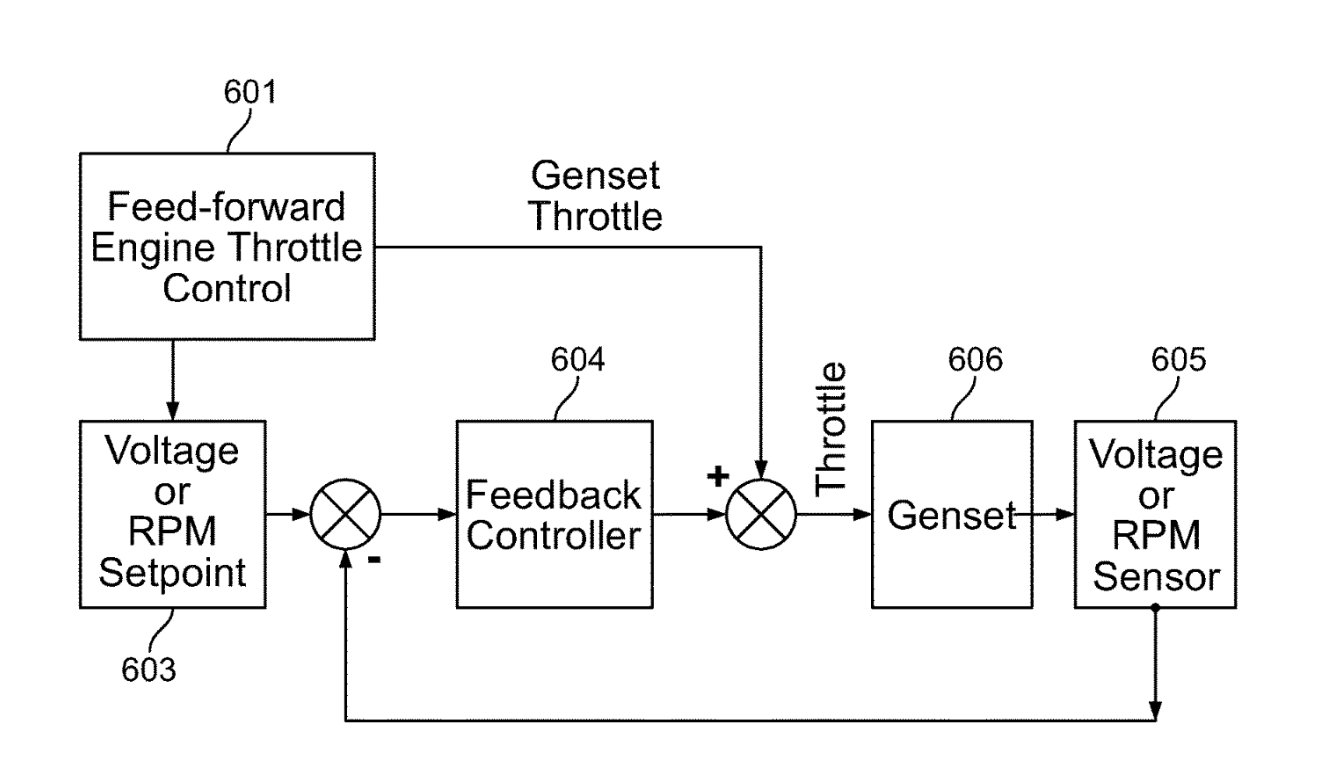
\includegraphics[scale=0.24]{patents/US10144527B2-fig6.png}
  \caption{Изображение взятое из патента US10144527B2}
\end{figure}

Полётный контроллер включает в себя, модуль управления двигателем с
обратной связью (601), источник опорного напряжения (603), контроллер
обратной связи (604), датчик напряжения или оборотов в минуту (605).

% https://patentimages.storage.googleapis.com/76/c7/4c/d47d31176792f4/US10144527.pdf

В ~\cite{TW202504822A} представлен беспилотный летательный аппарат
мультироторного типа, использующий умное устройство в качестве
полётного контроллера.

\begin{figure}[H]
  \centering
  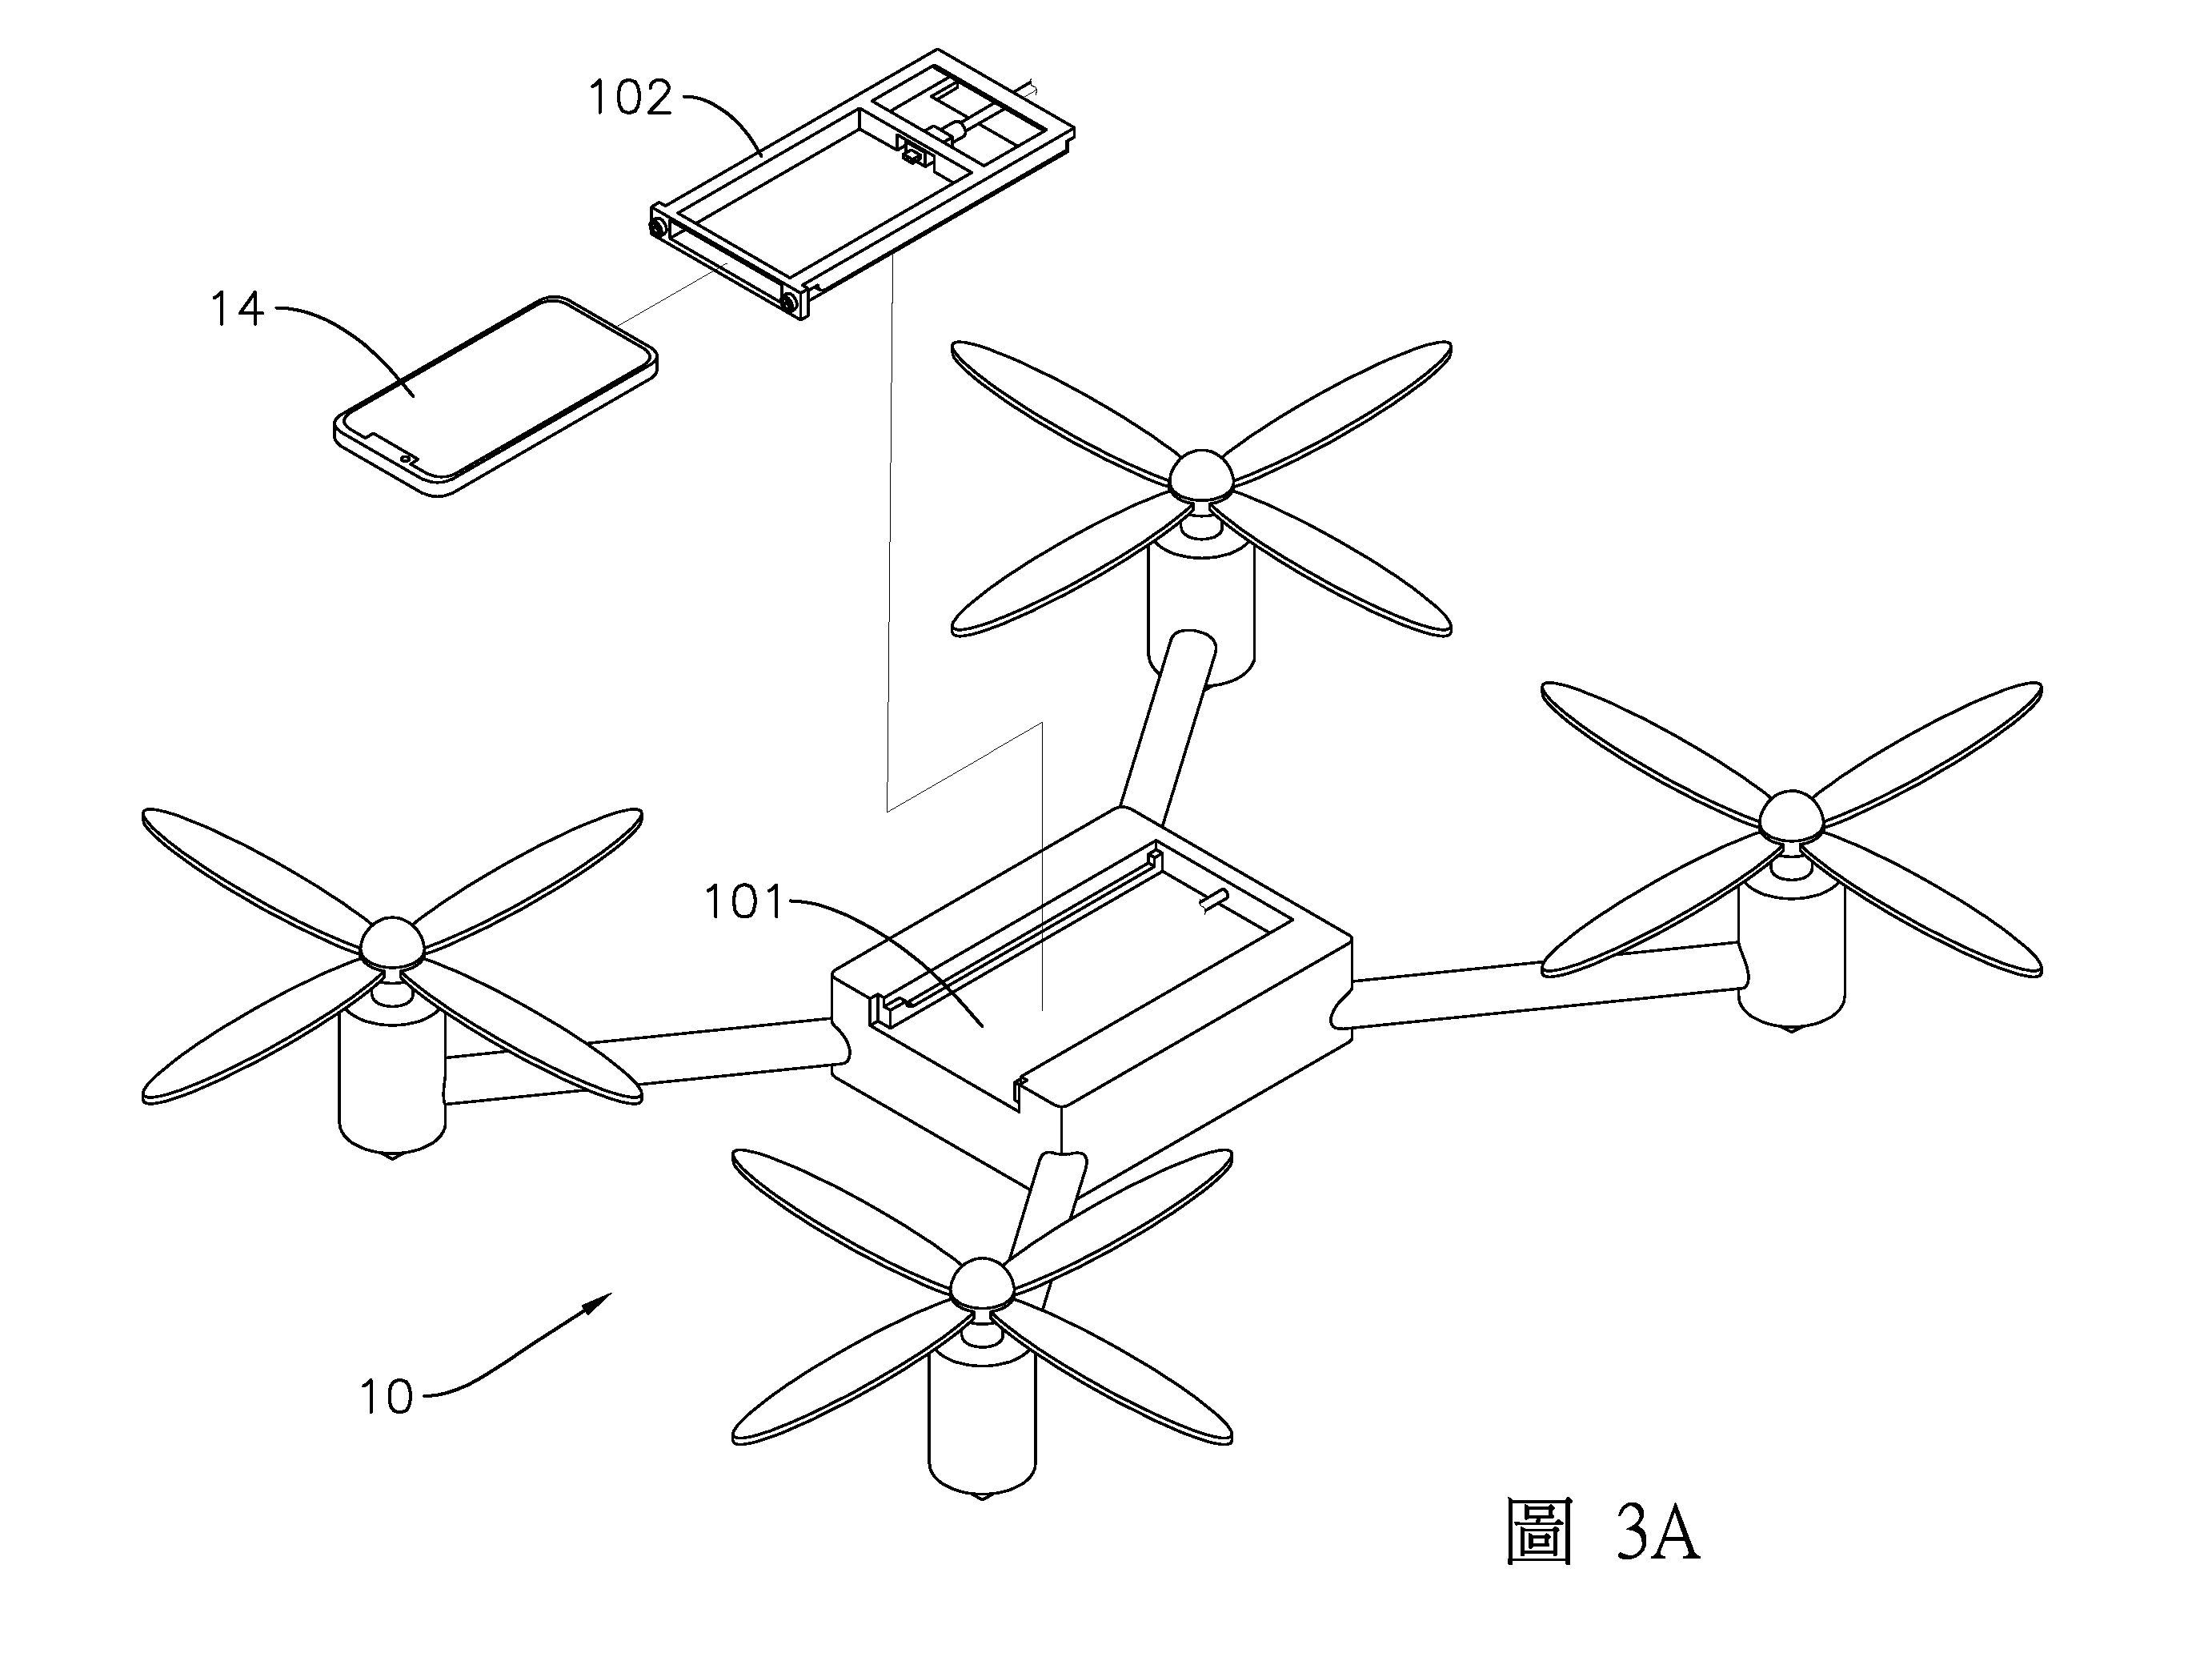
\includegraphics[scale=0.10]{patents/TW202504822A-fig4.png}
  \caption{Изображение взятое из патента TW202504822A}
\end{figure}

% https://patentimages.storage.googleapis.com/3e/92/7a/2f64a534cdc244/TW202504822A.pdf

Беспилотный летательный аппарат мультироторного типа включает в
себя фюзеляж (10), приёмный слот (101) для установки корпуса (102) для
умного устройства (14).

В ~\cite{US20210245877A1} представлен полётный контроллер с
синхронизированным алгоритмом взаимодействия между сенсорами и
актуаторами.

\begin{figure}[H]
  \centering
  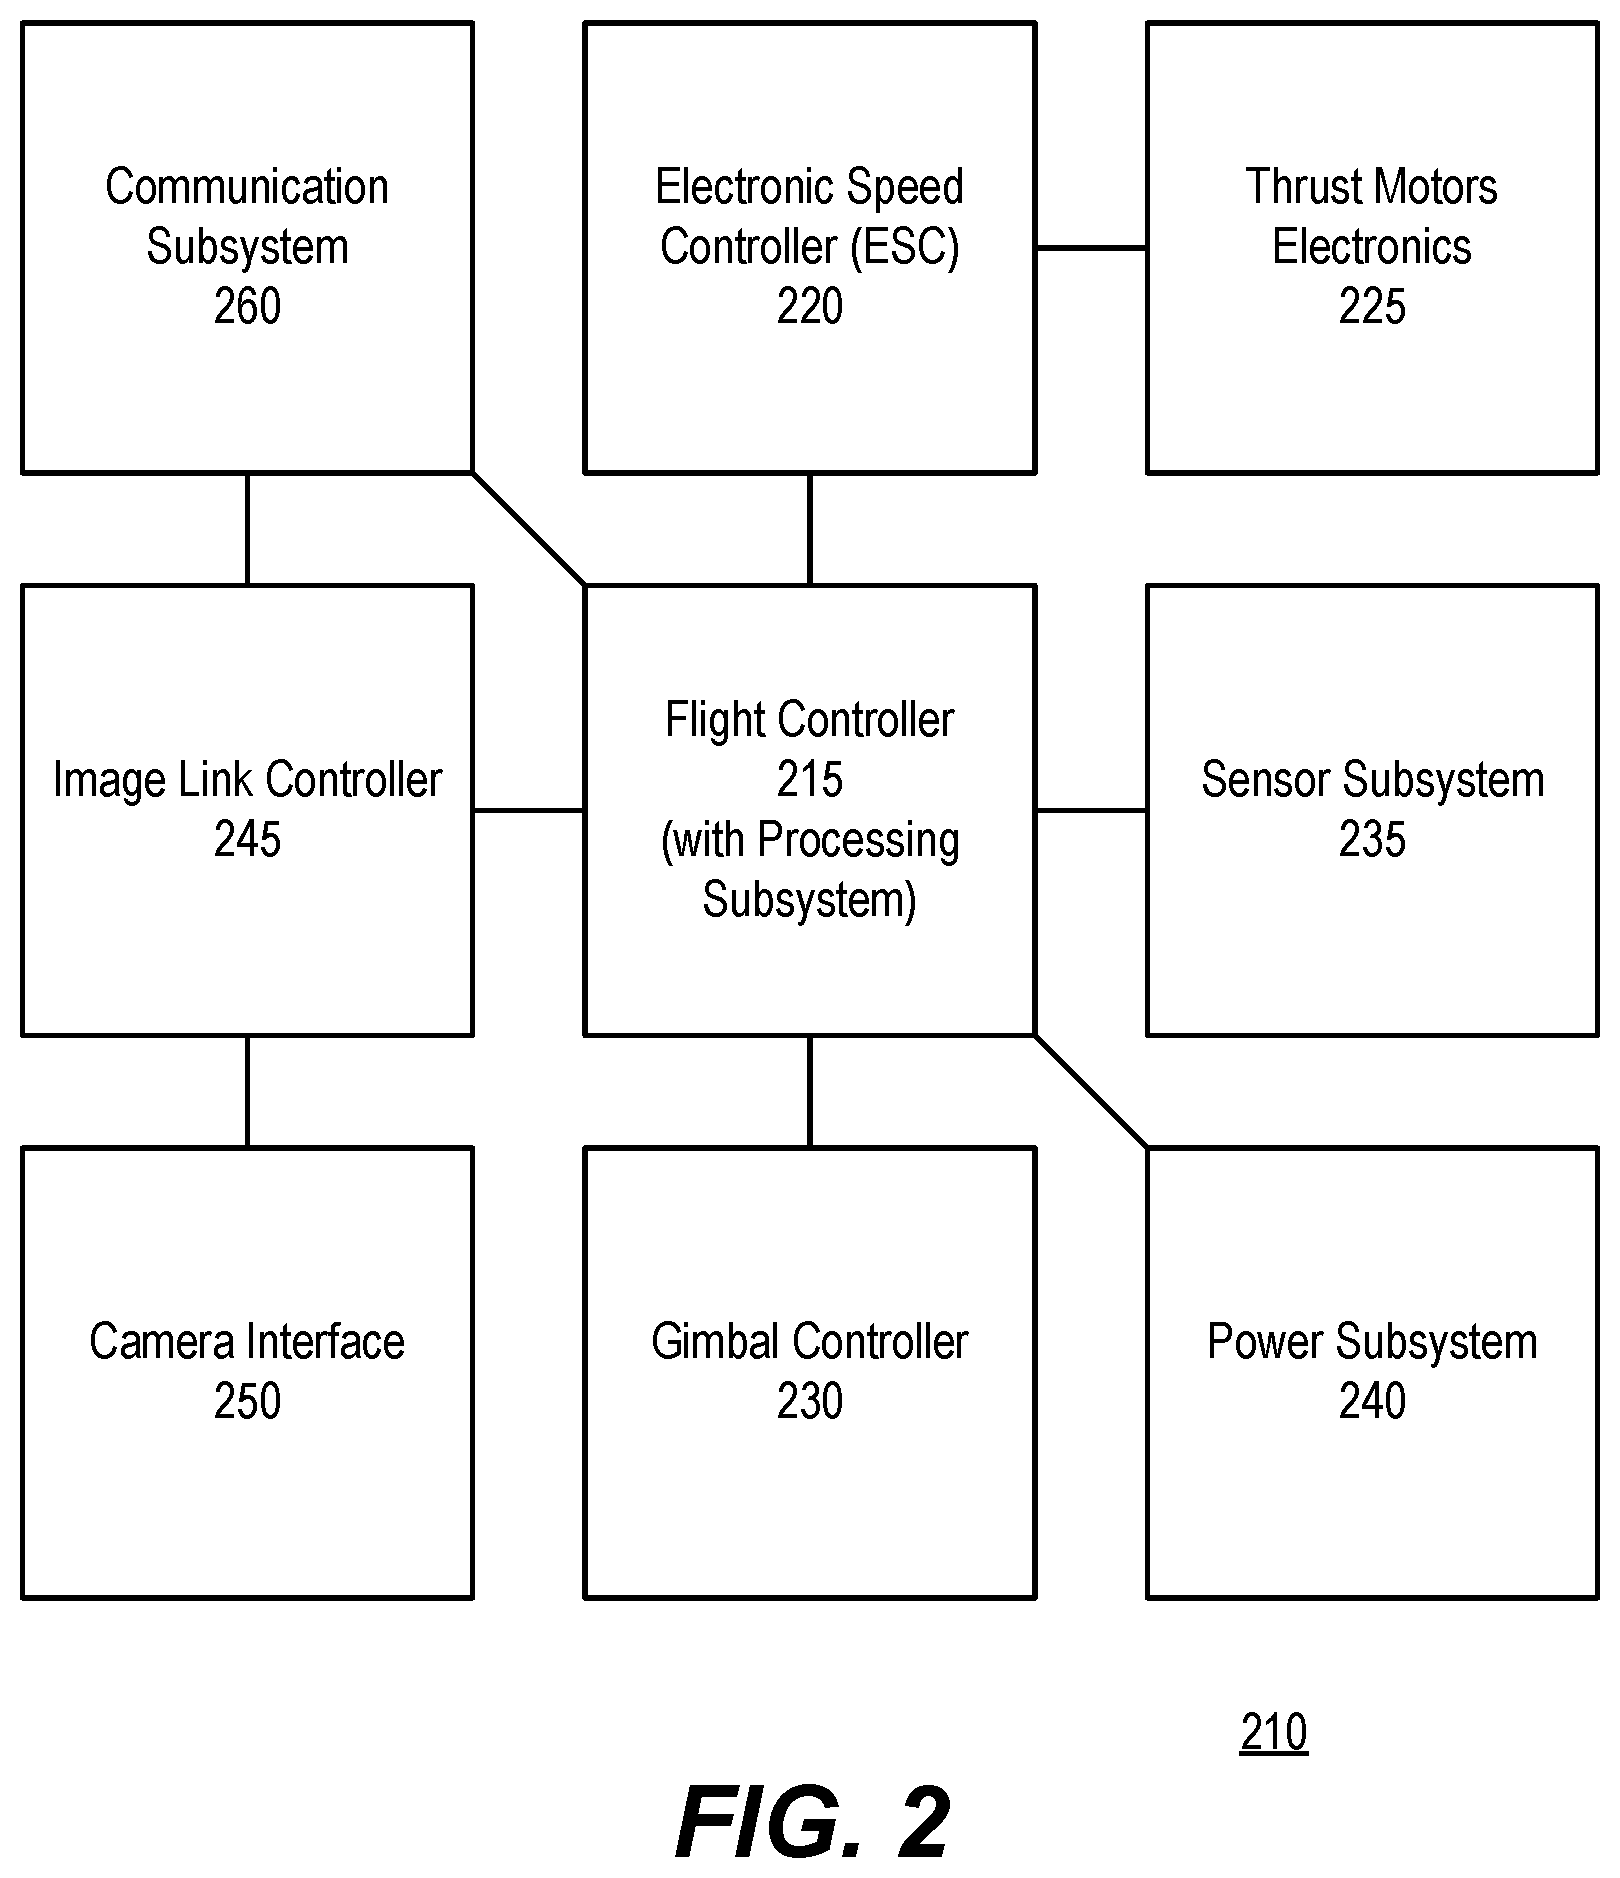
\includegraphics[scale=0.10]{patents/US20210245877A1-fig2.png}
  \caption{Изображение взятое из патента US20210245877A1}
\end{figure}

Система из беспилотного летательного аппарата мультироторного типа и
полётного контроллера(210) включает в себя полётный контроллер с
подсистемой обработки данных (215), электронный регулятор скорости
(220), электронику тяговых двигателей (225), подсистему датчиков
(235), подсистему питания (240), контроллер данных камеры (245),
интерфейс камеры (250), подсистему коммуникаций (260).

В ~\cite{US10551834B2} представлено электронное устройство для
управления беспилотном летательным аппаратом и соответствующий метод.

% \begin{figure}[H]
%   \centering
%   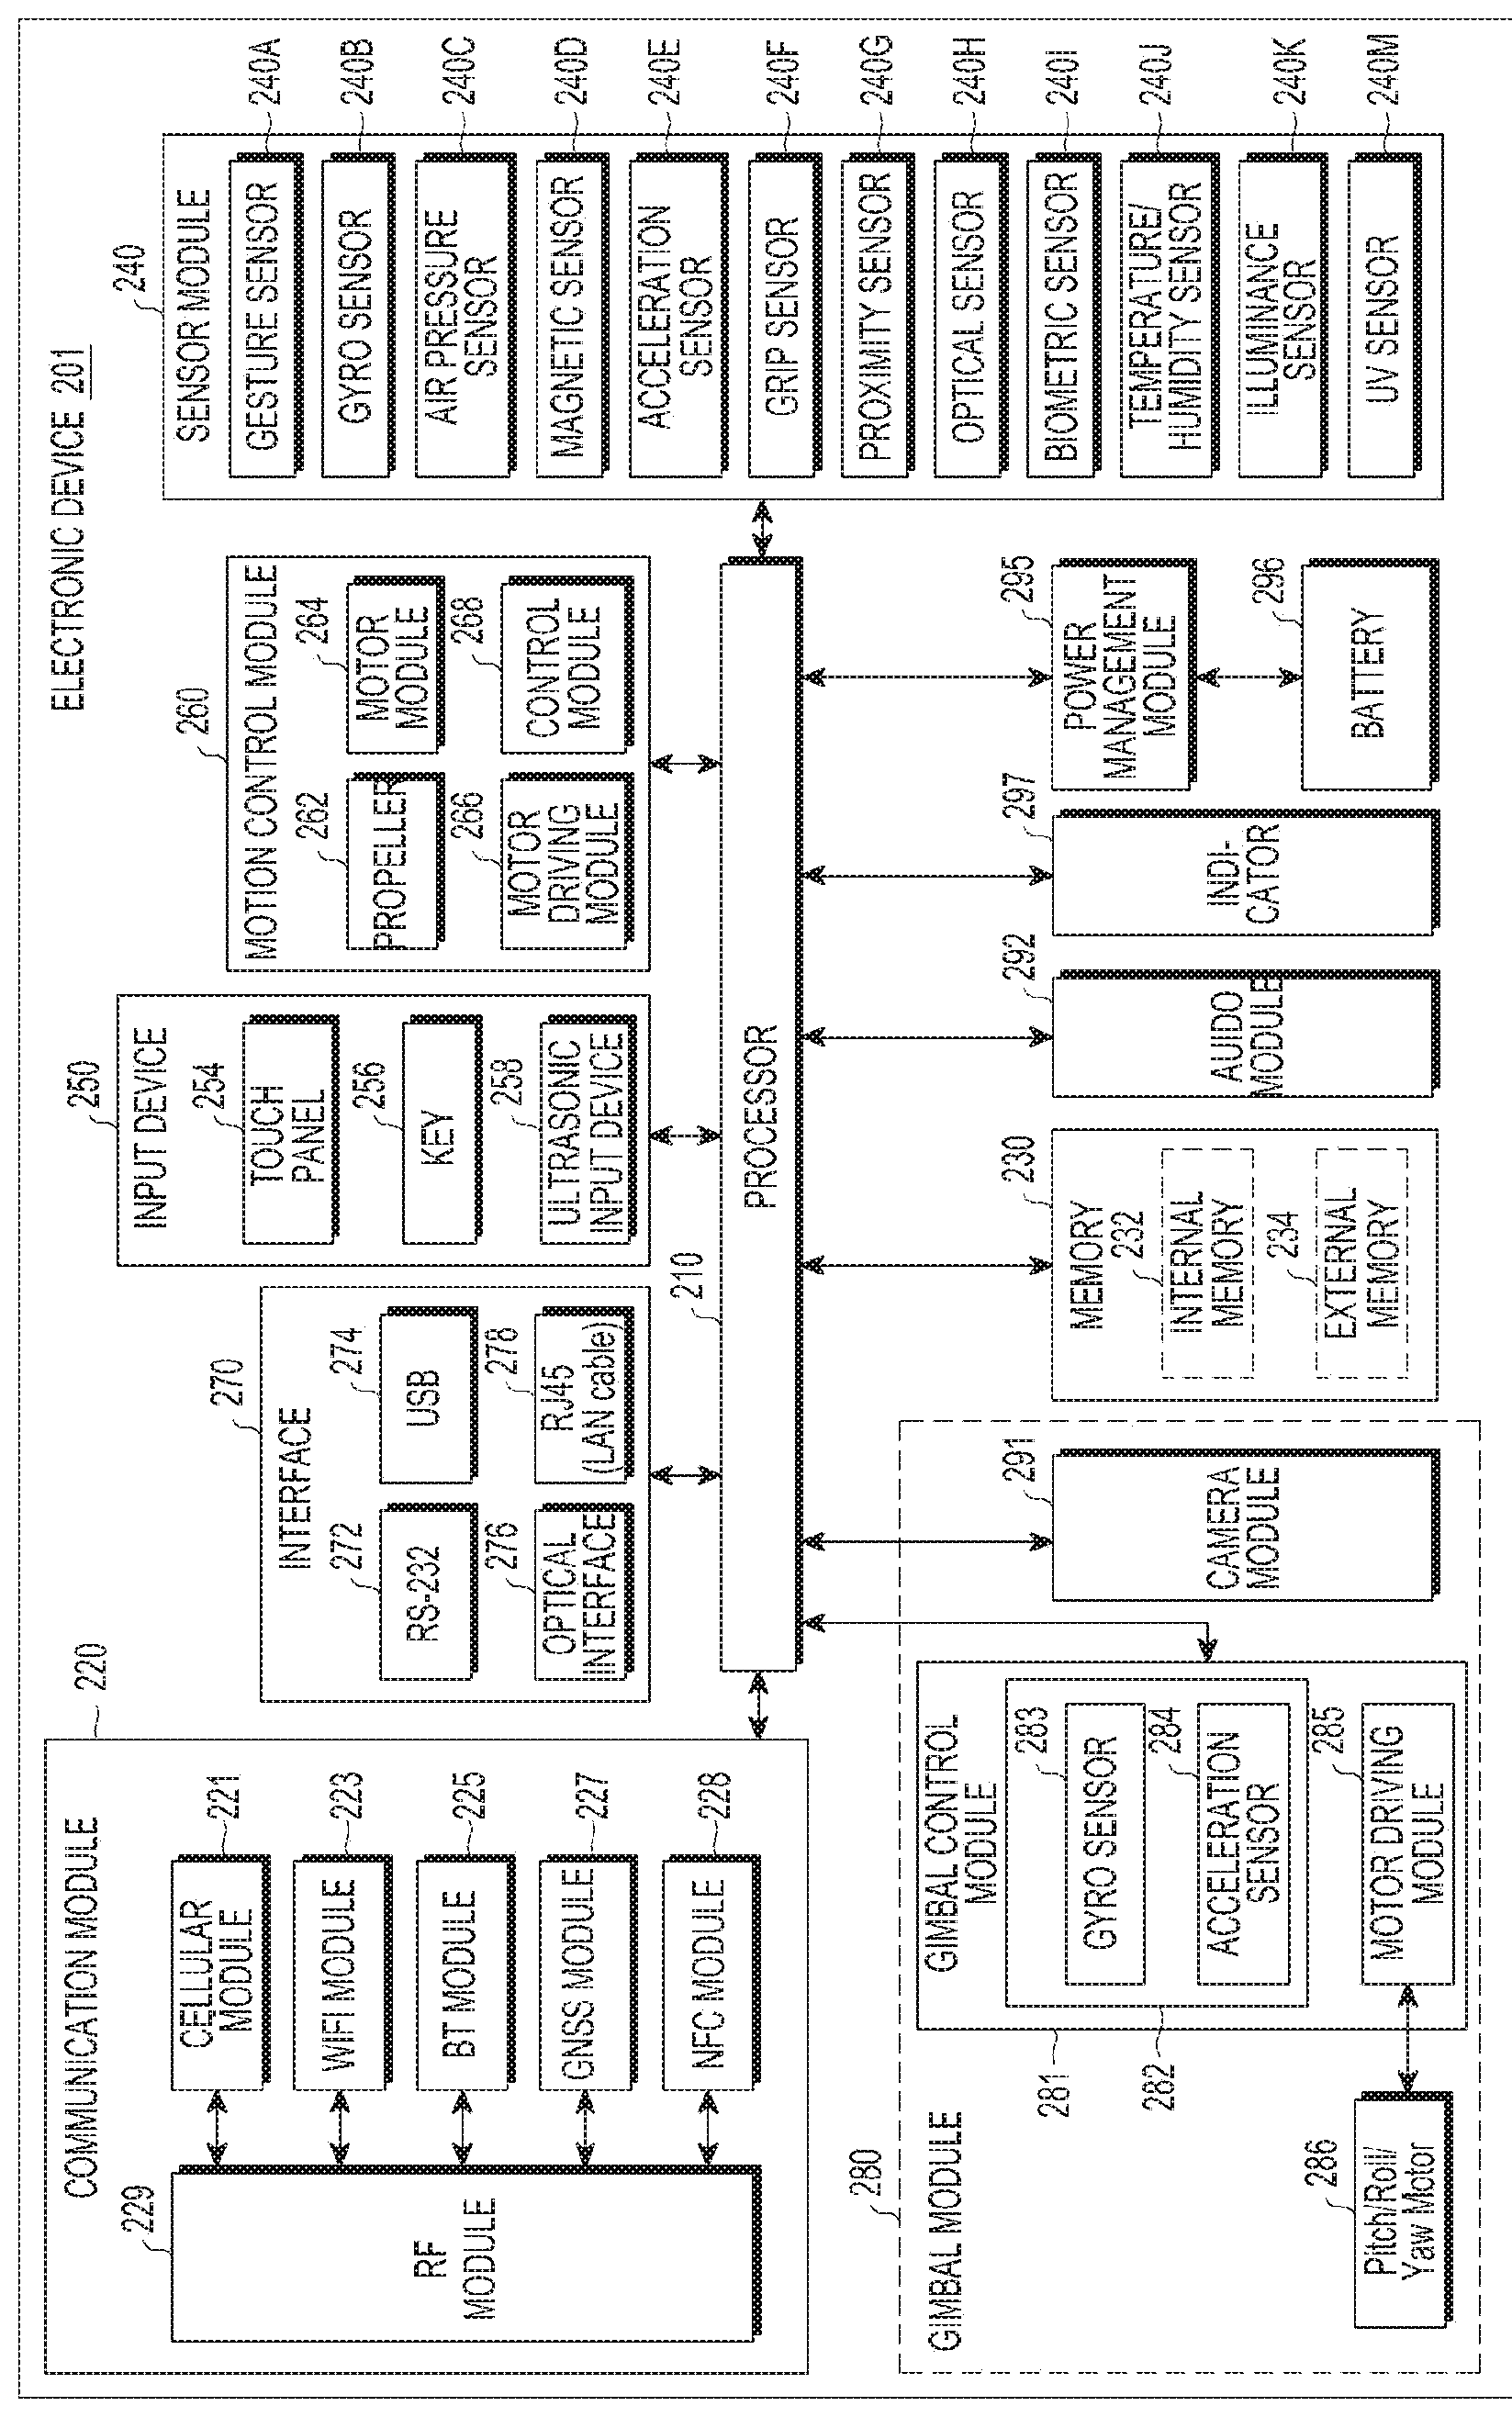
\includegraphics[scale=0.10]{patents/US10551834B2-fig2.png}
%   \caption{Изображение взятое из патента US10551834B2}
% \end{figure}

\newpage
%%% Local Variables:
%%% mode: LaTeX
%%% TeX-master: "main"
%%% End:
